\chapter{opdracht 3}

Bij deze opdracht worden LEDs van de bovenste 4 Rijen van de LED matrix van de microkit gedimd.
\begin{enumerate}[label=\Alph*.]
	\item In het onderstaande programma (listing \ref{lst:dimInp})wordt het middelste bit gedimd waarbij de
	$ duty cycle \text{Duty cycle} = \frac{10}{255} \times 100\% = 3.9\%$ is.
	De complete code  is te downloaden als \href{https://github.com/JohnVi-hhs/embsysP/tree/main/voorbeelden/dimOpdracht.ino}{voorbeeldcode \ref{lst:changeBut} van GitHub}
	\begin{lstlisting}[caption= Het dimmen van de LED,label={lst:dimInp}]
void setup() {  
	
	initMatrix();
	delay(1000);
	analogWrite(ROW3,10);
	
}

void loop(){
}

\end{lstlisting}
Laat de duty cycle in 15 stappen oploppen van 0\% naar 100\% hierna weer van 100\% naar 0| zoals te zien is in het \href{FadeInStapjesEnkeleLed.mp4}{filmpje}.
\item Laat in kolom 1, rij0 t/m rij3 het dimmen van de LED steeds minder worden, zoals te zien in figuur \ref{fig:dimledkol}.
\begin{figure}[h!]
	\captionsetup{justification=centering}
	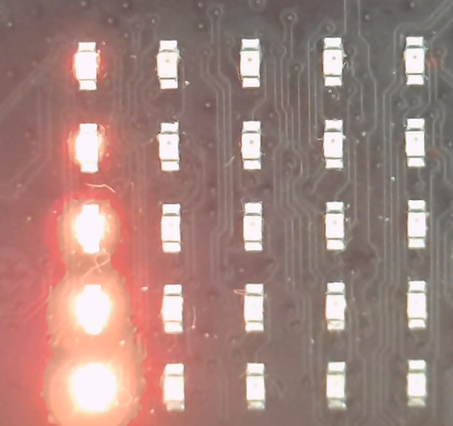
\includegraphics[width=0.3 \linewidth]{figuren/dimledkol}
	\centering
	\caption{Het dimmen van de LEDs in één kolom.}
	\label{fig:dimledkol}
\end{figure}
\item Laat de gedimde kolom continu langs alle kolommen gaan, zoals te zien is in het volgende \href{FadeKolommen.mp4}{filmpje}.
	
\item Laat de LED om 1 rij dimmen zoals te zien is in figuur \ref{fig:rijDimLed}
\begin{figure}[H]
	\captionsetup{justification=centering}
	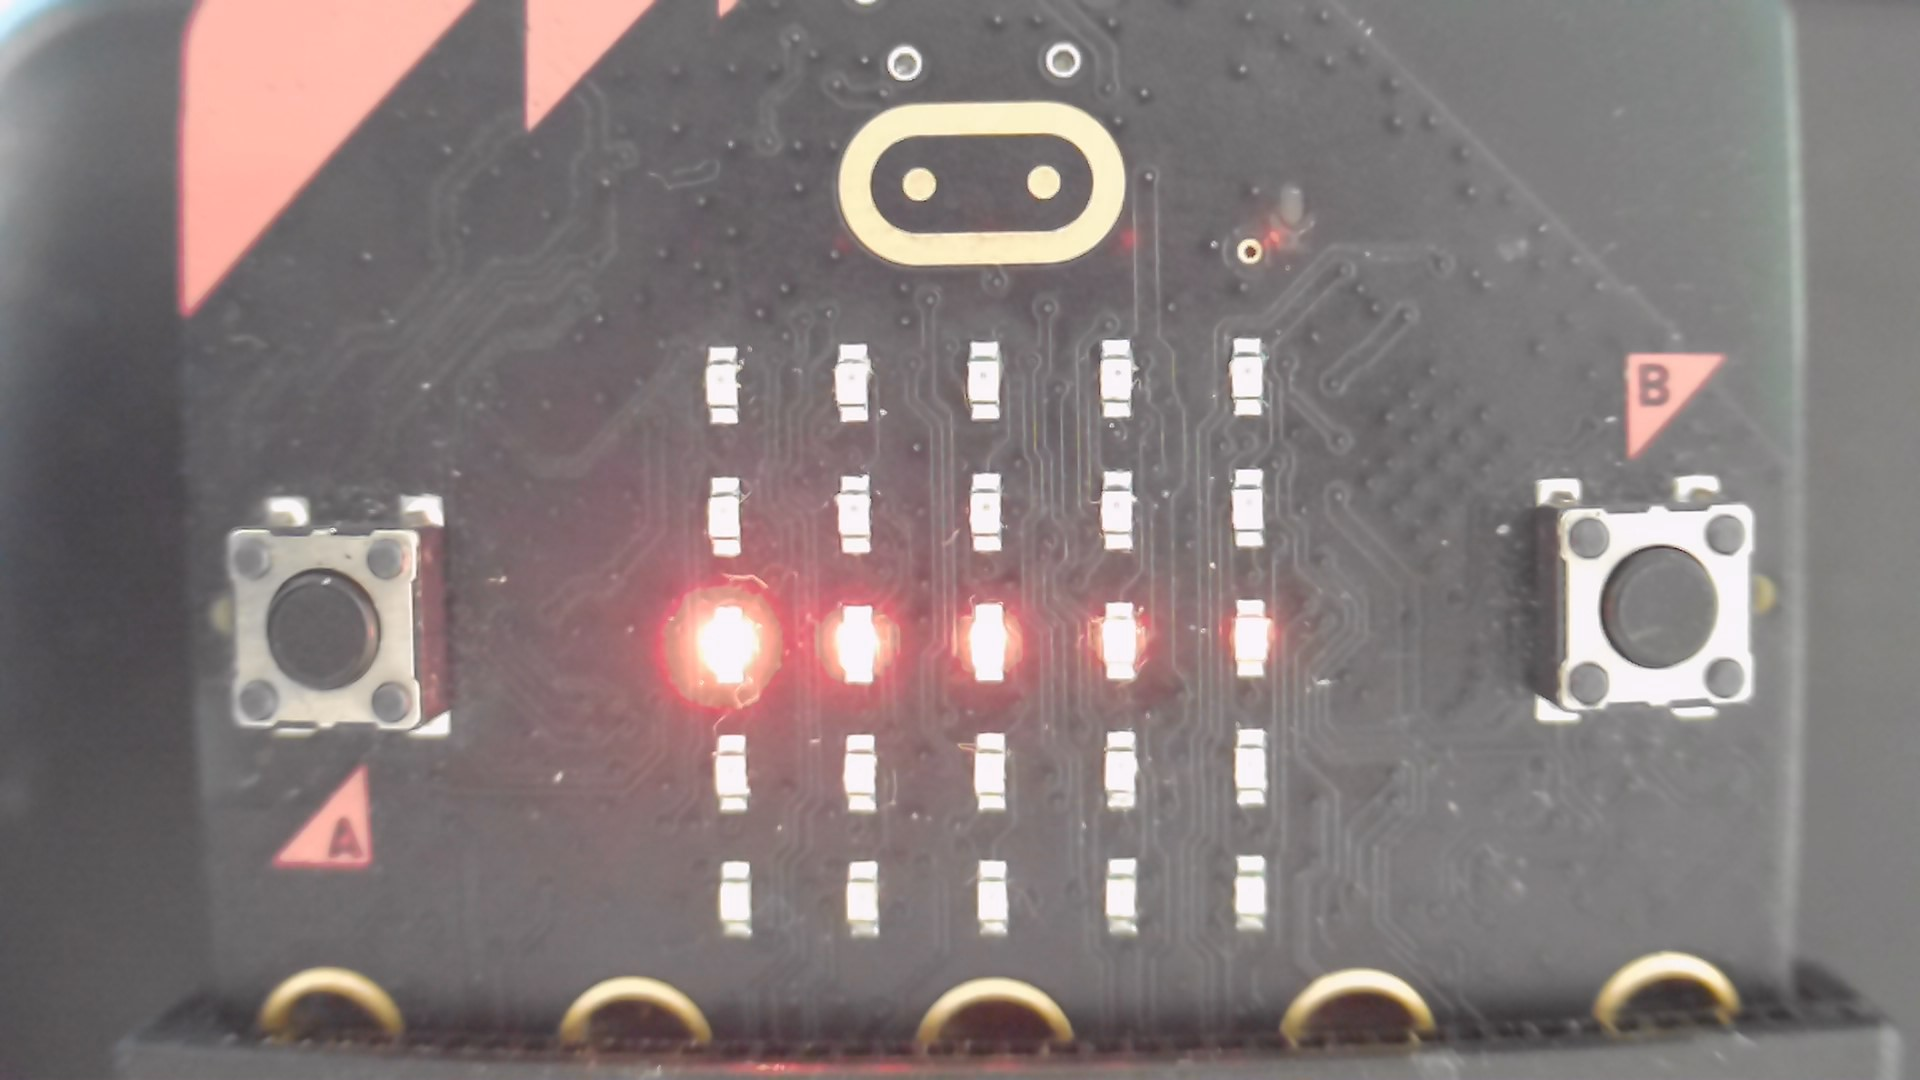
\includegraphics[width=0.3 \linewidth]{figuren/rijDimLed}
	\centering
	\caption{Het dimmen van de LEDs in één rij.}
	\label{fig:rijDimLed}
\end{figure}

\item Laat de rij van de gedimde rij leds continu rond draaien zoals te zien in het het volgende 
\href{FadeRijen.mp4}{filmpje}.
\end{enumerate}

